\subsection{Description}
This experiment is to assess importance of careful memory management in multithreading of Rust. 
In Rust programming, we usually need Atomic Reference Counting (Arc) to share data among threads. 
Arc is a simple interface that allows threads to share data, but it may cause significant overhead in Big Data processing.
Arc allows multiple variable to have ownerships of a particular value similarly to Rc, 
but also supports atomic feature enabling the ownerships exist in different threads. 

As explained in last experiment, deletion of Rc has significant overhead than normal reference. 
By learning this result, our assumption is that deletion of Arc has also overhead when we compare to normal reference. 
In many situation where developer write a multithreading code, Arc is used and the deletion happens multiple times. 
To assess runtime overhead of algorithm with Arc, We implement merge-sort algorithm in two different ways. 
One is sharing source vector with Arc. The other is passing slice of source vector to child thread. 

Our merge-sort algorithms are implemented with recursion. For each call of recursive function, 
Arc or slice of the source vector needs to be passed and deleted when the function returns value. 
These merge-sort algorithms trigger large number of Arc or reference deletion proportional to the number of call recursive function.
Merge-sort algorithm can be separated in three phases: splitting phase, copying phase, and merging phase. 

The splitting phase is merely acquiring index of range. At this phase, multiple threads are generated and Arc or reference of source vector are passed by calling recursive function. 
Copying phase occurs in the base case of the recursive call. The element in the source vector in a certain index is deep-copied into newly allocated vector.
At merge phase, merge function receives two sorted independent vector and merge them into single new vector.

We use scope method from crossbeam crate to perform multithread programming. 
Scoped thread can have reference to value from its parent thread by ensuring children threads are joined before their parent thread returns value. 
By using scoped thread, we can implement two merge-sort algorithms in identical way except whether the function receives Arc or reference of source vector.
The representations of source vector for each algorithm are shown in figure.

\begin{figure}[htb]
    \begin{lstlisting}
        // Source vector for algorithm with Arc.
        arr: Arc<VecDeque<T>>

        // Source vector for algorithm with reference (slice).
        arr: &[T]
    \end{lstlisting}
    \caption{Representation of Source Vector}
    \label{fig:Sampling}
\end{figure}


\subsection{Result}
The elements of source vector are CustomerOwned objects. We generates source vectors in size of 1 million, 2 million, 3 million and 4 million. 
Finally, merge-sort is performed based on Customer key value. The figure shows the result for runtime performance of merge-sort algorithms on difference size of vectors.

\begin{figure}[htb]
    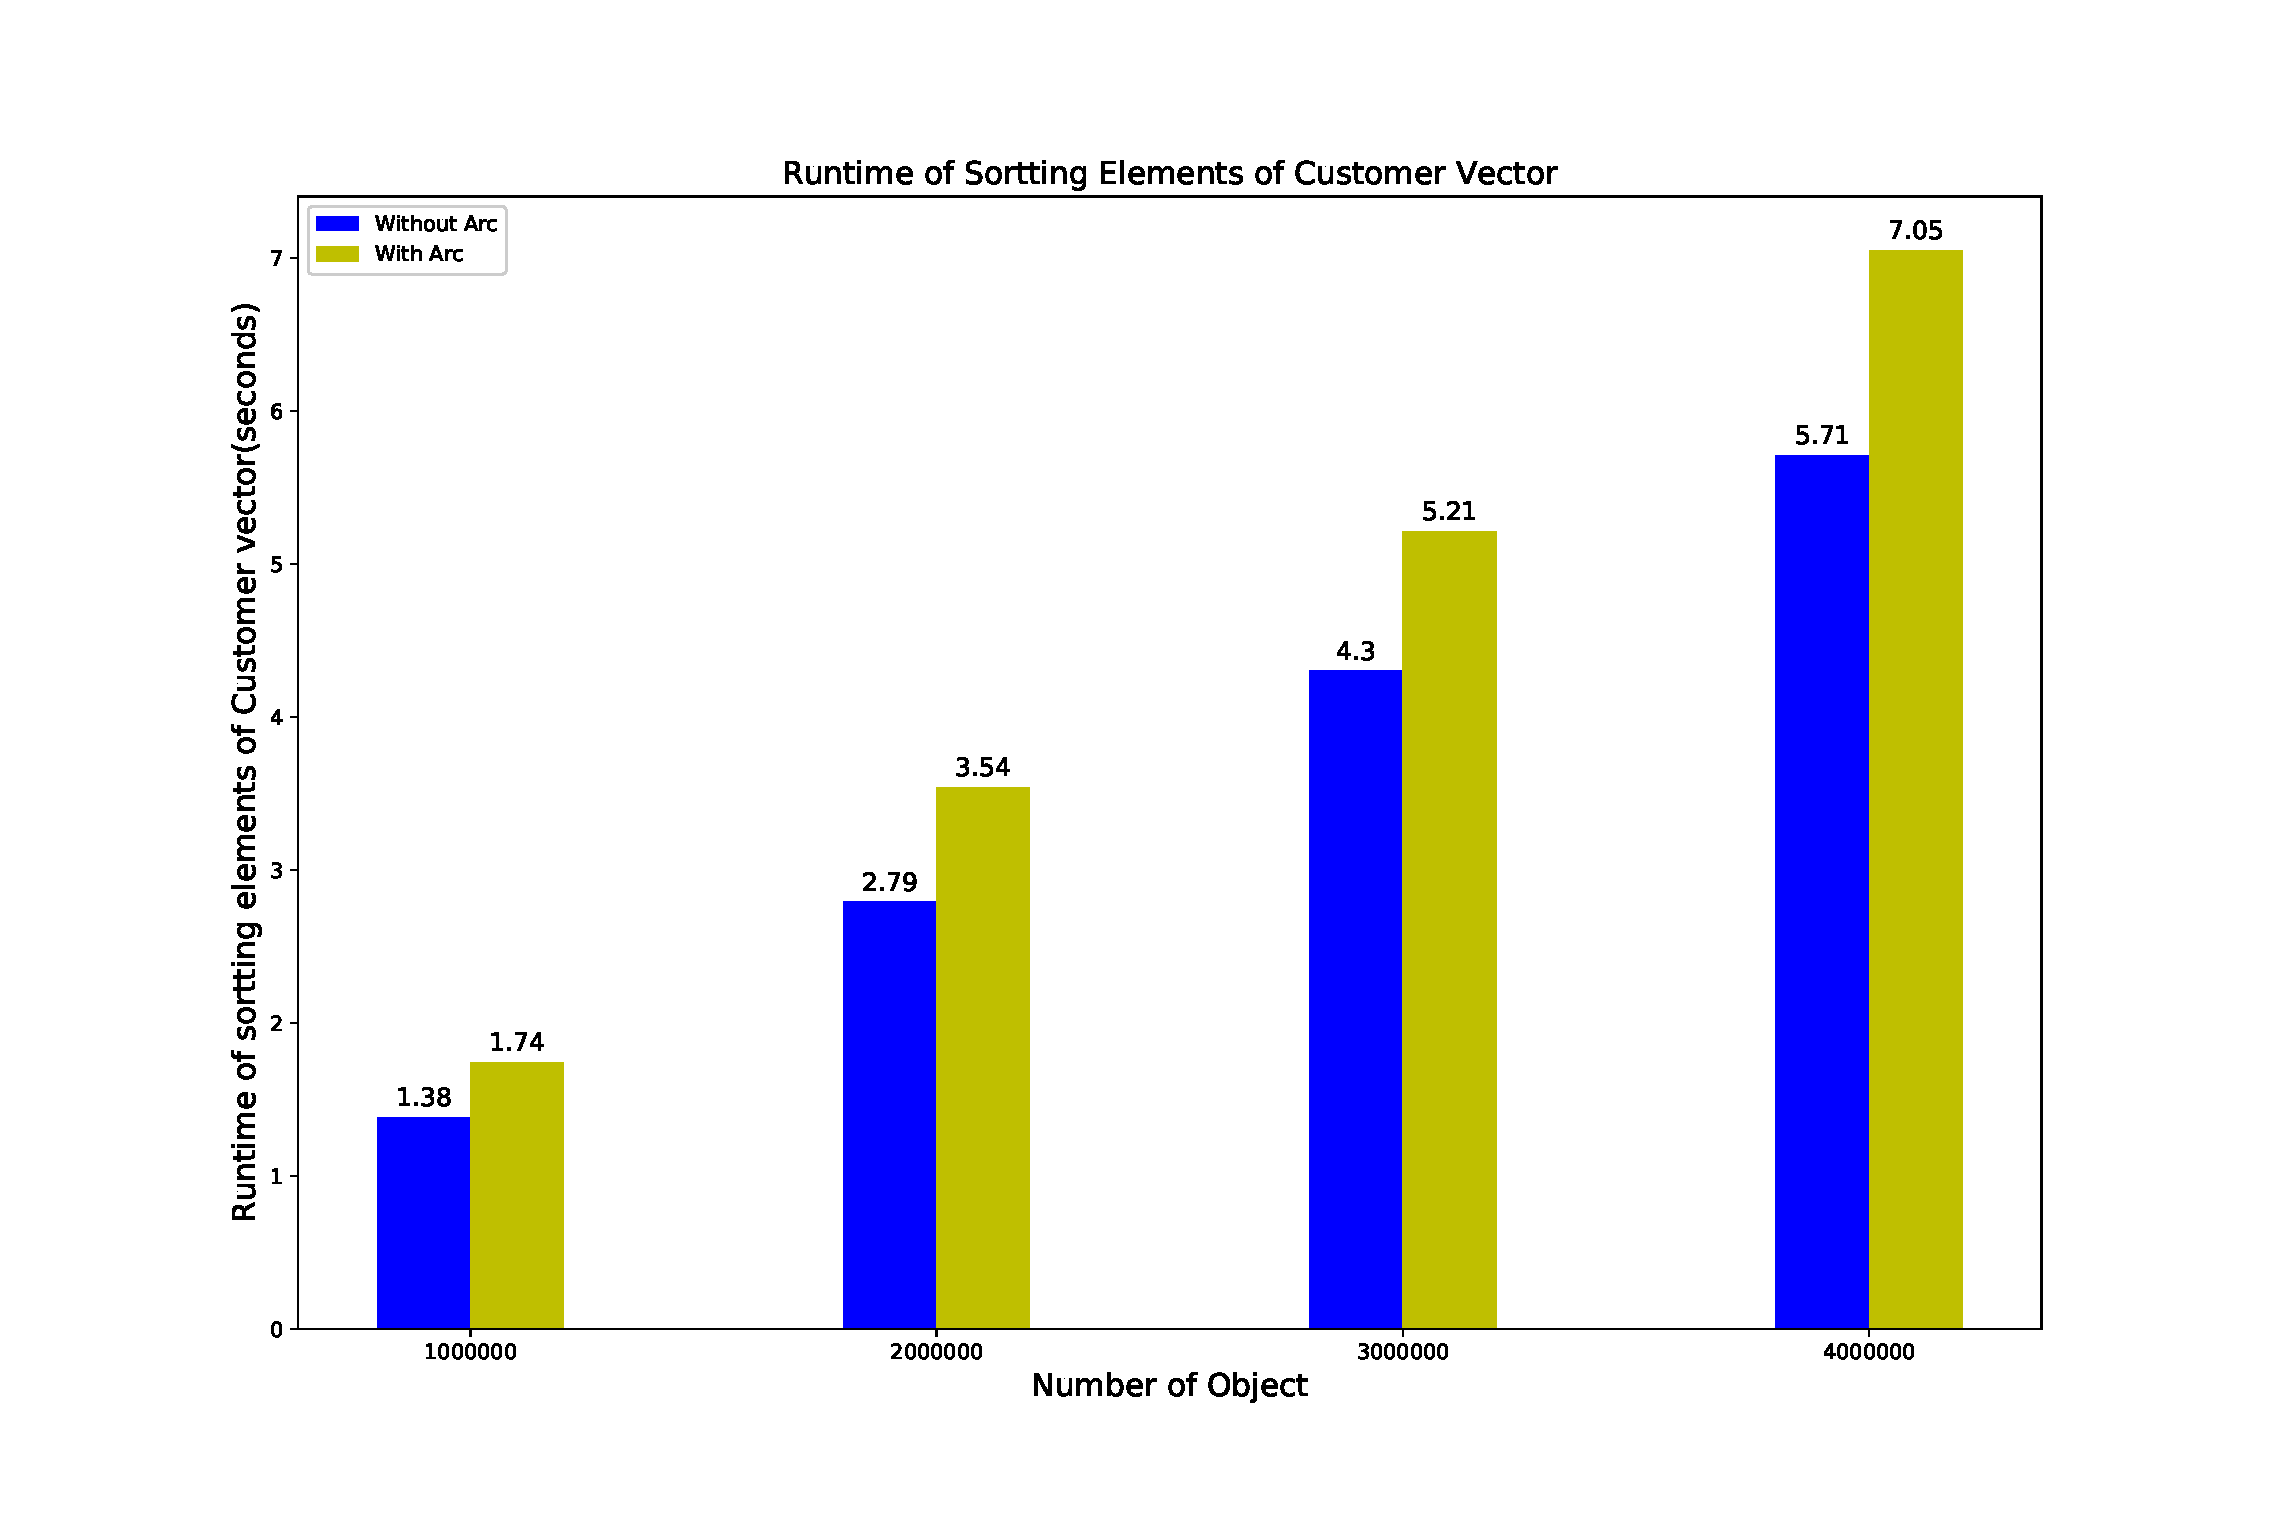
\includegraphics[width=15cm]{rust_merge_sort.eps}
    \caption{Runtime of Sortting Elements of Customer Vector}
    \label{fig:Sampling}
\end{figure}

\subsection{Discussion}

